\chapter{Design}

I dette kapitel beskrives design-delen af hardware og software for SRM. På baggrund af arkitekturen redegøres der, hvordan HW/SW-blokkene, som indgår i arkitekturen er designet samt deres funktion. Designet for HW-delen indeholder diagrammer samt beregninger af komponentværdier. Desuden indeholder HW-delen en kort
beskrivelse af designovervejelser i forhold til de enkelte hardwareenheder. SW-designet beskriver funktioner og GUI samt særligt interessante dele af den interne logik i funktioner. 


\section{Hardware}

Dette afsnit omhandler designet af hardwaren, som anvendes til at måle  bioimpedans- og EMG-siganler. Figur \ref{fig:Blokaede} viser de komponenter, som skal anvendes for at SRM kan blive realiseret. SRM består af både designet komponenter og kommercielle komponenter. Ved designet komponenter er der prioriteret komponenter som var tilgængelige på lokalt elektronikværksted. Udover krav til de individuelle komponenter, er alle komponenter valgt efter at kunne håndtere en eksitationsspænding på $\pm$18 V. Disse kommercielle komponenter omfatter en Analog Discovery, en pc, en EMG-måler og er ikke blevet designet. Der er i stedet for lagt vægt på om de kan leve op til de krav, som er nødvendige for at realisere det ønskede produkt.


\begin{figure}[H]
\centering
{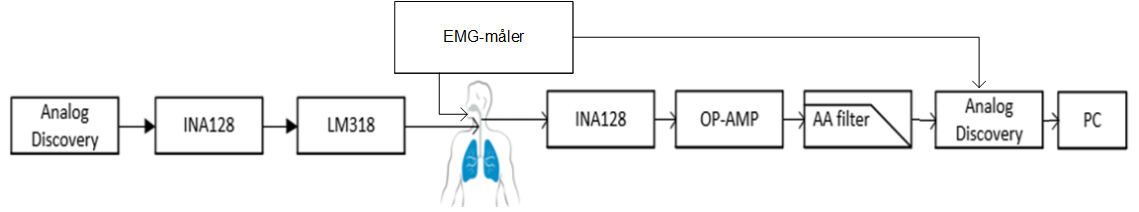
\includegraphics[width=\textwidth]
{Figure/Blokaede}}
\caption{Figuren viser de enkelte komponenter, som skal designes for at realisere SRM.}
\label{fig:Blokaede}
\end{figure}

\subsubsection{Analog Discovery}

AD har i dette bachelorprojekt to formål, at fungerer som funktionsgenerator og som dataopsamlingsmodul. Figur \ref{fig:ADogINA128} viser disse to formål. Det ene formål er at funktionsgeneratoren laver et AC signal med ampiltuden på 2 V og 20 kHz, som sendes til indgangen af instrumentationsforstærkeren INA128. Signalet bliver brugt til at generere en konstant strøm ud af operationsforstærkeren LM318N. Det andet formål er at AD modtager signal fra anti-aliaseringsfilter, som bliver konverteret fra analogt til digitalt signal.

\begin{figure}[H]
\centering
{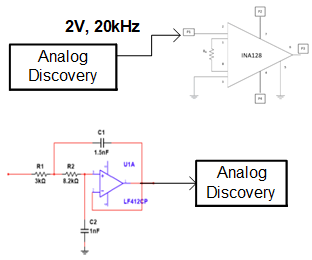
\includegraphics[width=10cm]
{Figure/ADogINA128}}
\caption{Figuren viser AD's funktion i det samlede system. AD fungerer som funktionsgenerator og som dataopsamlingsmodul.}
\label{fig:ADogINA128}
\end{figure}

Generelt for at foretage korrekt dataopsamling af signalet fra analogt domæne til digitalt domæne, skal Shannons samplingsteori overholdes. Det vil sige at samplingsfrekvensen skal minimum være det dobbelte af den maksimale frekvenskomponent, Nyquist-frekvensen. Frekvenser større end Nyquist-frekvensen giver anledning til aliasering. Dette vil resultere i et fejlsignal. Derfor vælges der en samlingsfrekvens som er væsentlig højere end den maksimale frekvenskomponent. 

Valg af dataopsamlingsenhed har også betydning for overgangen fra analogt domæne til digitalt domæne. Her konverteres de analoge værdier til de nærmeste digitale værdier. Konverteringen bestemmes af ADC'ens spændingsområde og opløsning. Forholdet i mellem spændningsområde og opløsning, udtrykkes LSB. LSB er et udtryk for den mindste detekterbare spændningsændring som ADC'en kan detektere. I henhold til AD's datablad, se \nameref{bilag15}, er denne opløsning på 14 bit, samtidig med et spændningsområde på 8 V, resulteret i en mindste spændningsændring som AD kan detektere 0,48 mV. Der henvises til \nameref{bilag5}, for den fulde udregning af LSB.

Derfor er det besluttet at bruge AD, da den har følgende fordele:
\begin{itemize}
\item Den kan fungere som funktionsgenerator samtidig med, at den læser to signaler ind simultant
\item Den kan sample to signaler simultant med en samplingsfrekvens på 500 kHz
\item Den kan fungere som dataopsamlingsenhed
\end{itemize}



\subsubsection{Instrumentationsforstærker}

Instrumentationsforstærkeren i dette bachelorprojekt, har til formål at undertrykke støj fra måleobjekt og efterfølgende forstærke signalet, men også forstærke indgangssignalet fra AD's funktionsgenerator. Derfor anvendes i dette
projekt to instrumentationsforstærker af typen INA128P. INA128P specifikationer kan læses i \nameref{bilag15}. INA128P giver mulighed for at forstærke signalet vha. kun en modstand. Fordelene ved anvendelse af instrumentationsforstærker, når det ønskes at måle elektrofysiologiske signaler er\cite{PeterJohansen2014}:
\begin{itemize}
\item 	Høj indgangsimpedans på ca. $10^{10} \Omega $
\item	Stor common mode rejection (CMR) på minimum 120dB
\item 	Differentielt input-single ended out (nødvendigt for at mindske $CM_{noise}$)
\end{itemize}



\textbf{Instrumentationsforstærker 1}

Den ene INA128 benyttes til at forstærke signalet og undertrykke støj fra AD's funktionsgenerator. Det ønskes at forstærke de 2 V fra AD til 4 V. Det vil sige at gain er 2 og derfor kan R$_{G}$ modstanden beregnes til 50 k$\Omega$. Udregning af R$_{G}$, diagram og stykliste kan ses i \nameref{bilag5}.

\textbf{Instrumentationsforstærker 2}

Den anden INA128 anvendes til at forstærke elektrofysiologiske signaler fra måleobjektet og undertrykkelse af commen mode støj. Det ønskes at INA128 forstærker med 100 gange, da det forventes at den målte spændingsforskel ligger i milli- og mikrovolt området\cite{PeterJohansen2014}. 

For at denne forstærkning på 100 gange kan lade sig gøre, er det nødvendigt at slå op i databladet til INA128. Det kan konstateres at med en gain på 100, er det muligt at gå op til 100 kHz, hvilket fint stemmer overens da denne båndbredde  ligger over anti-aliaseringsfilterets knækfrekvens på 25 kHz. Det er nu muligt at udregne R$_{G}$ modstand, til 505 $\Omega$. Til en fremtidig modultest af INA128's forstærkning, blev der designet en spændingsdeler til formålet. Udregning af R$_{G}$, diagrammer, stykliste og spændingsdeler kan ses i \nameref{bilag5}.

 
 
\subsubsection{Strømgenerator}
Strømgeneratoren i dette bachelorprojekt, har til formål at generere en strøm til måleobjektet gennem elektroderne. Dette er et krav for at kunne udføre en bioimpedans måling på et måleobjekt\cite{Brantlov2017}. 

Strømgeneratoren også kaldet VCCS er designet efter en basis Howland pumpe. Ved udvælgelse af operationsforstærker kigges der på slewrate som skal overholdes. For at udregne slewrate bruges 20 kHz og 4 V. Slewrate udregnes til 0,503 V/$\mu$s. Her vælges operationsforstærkeren LM318, da den oplyses i databladet til at have en slewrate på 70 V/$\mu$s og den består kun en operationsforstærker. Den forventet strøm blev udregnet til 283 $\mu$A. Udregning af Howland pumpen, slew rate, diagram og stykliste kan læses i \nameref{bilag5}.


\subsubsection{OP-AMP}
OP-AMP i dette bachelorprojekt, har til formål at forstærke output signalet fra Instrumentationsforstærker 2. Der er valgt at benytte en ikke-inverterende operationsforstærker. Det ønskes at den forstærker op for at udnytte AD inputområde, som ligger mellem $\pm$25 V. 

Signalet forstærkes op til 10 V, hvor gain udregnes ud fra forholdet mellem to modstande i OP-AMP kredsløbet. Den ene modstand sættes til 1 k$\Omega$ og den anden modstand udregnes til 9 k$\Omega$. Slew rate udregnes til 1,257 V/$\mu$s. Igen vælges operationsforstærkeren LM318, da den oplyses i databladet til at have en slewrate på 70 V/$\mu$s og den består kun en operationsforstærker. Udregninger af gain modstande og slew rate samt diagram og stykliste findes i \nameref{bilag5}.


\subsection{AA filter}

AA filter i dette bachelorprojekt, har til formål at dæmpe alt over den halve samplingfrekvens (Nyquist frekvensen). Samplingfrekvensen vælges til 500 kHz, derfor bliver Nyquist frekvensen 250 kHz. AD er en 14 bit ADC, hvilket stiller krav om at signalet ved 250 kHz skal være dæmpet under $1/2*LSB$, som i dB svarer til en dæmpning på $20log*2^{15}=90dB$. På baggrund af spektrumanalysen i modultesten som står i \nameref{bilag6}, er signalet aflæst til sig selv til at have en dæmpning på ca. 75 dB. Derfor ønskes at AA filter leverer en yderligere dæmpning med 20 dB. Dette anti-aliseringsfilter designes så det tillader passering af frekvenser, der er mindre en Nyquist frekvensen og dæmper frekvenser som er højere. Den yderligere dæmpning kan lade sig gøre med et første orden filter, da de dæmper med 20 dBpr. dekade. Dog vælges i stedet et 2. orden filter, der vil dæmpe 40 dB pr. dekade, da dette vil tage højde for eventuelle variationer i signalet når det optages. Det skal bemærkes at dette filter ikke påvirker det amplitude moduleret signal (synk) som ligger ved 20 kHz, da det stadig er indenfor for passbåndet og derfor ikke blive filteret væk.

AA filteret designes derfor med følgende specifikationer:
\begin{itemize}
\item Aktivt lavpas
\item 2. orden Butterworth
\item Sallen key
\item Knækfrekvens = 25 kHz
\end{itemize}

På baggrund af specifikationerne er disse indtastet i programmet FilterPro. Dette resulterer i et design med komponent værdier, stykliste og diagram over filteret. 

Her foretages to yderligere udregninger slew rate og GBWP for at bestemme den korrekte operationsforstærker. Slew rate udregnes til 1,257 V/$\mu$s og GBWP til 2,5 Mhz. Her vælges operationsforstærker OP27G, da der i databladet kan aflæses i slew rate på 2,8 V/$\mu$s og GBWP på 8 MHz. Hvilket stemmer fint med de udregnet værdier. Derudover er OP27G kendt fra tidligere semesterprojekt, hvor denne også skulle fungere som et lav pas filter. Udregningerne for AA filter, bodeplot, stykliste samt diagram kan læses i \nameref{bilag5}.


\section{Software}

Desuden indeholder bilaget et sekvens
diagram, der giver en detaljeret beskrivelse af udvalgte funktioner/metoder, som styrer
SRM hardware del.